\chapter{Implementacja algorytmów}
\label{sec:implementation}

W rozdziale tym opisana została implementa oraz wyniki pomiarów algorytmów dla przewidzianych środowisk oraz metod akceleracji (tabela \ref{tab:implemented}). Na początku opisana została organizacja plików projektu oraz sposób budowania bibliotek. Następnie omówione zostały wyniki detekcji z~wykorzystaniem transformacji Hough'a, które powinny być spójne dla wszystkich implementowanych metod akceleracji. Wszelkie problemy i~różnice wyników pomiędzy implementacjami poszczególnych metod opisane zostaną w~rozdziale \ref{sec:methods-results}. 

%oraz wyniki testów wydajności relatywnie do wykonania wariantu sekwencyjnego. 

%Na końcu omówiono przykład rzeczywistego użycia i~porównano wszystkie wyniki pomiarów.

\section{Organizacja plików}

Jednym z~założeń tej pracy jest analiza metod budowania bibliotek, które wykorzystują badane metody akceleracji obliczeń. Projekt, w~którym znajdują się zaimplementowane metody, został zbudowany w~oparciu o~strategię \textit{monorepo}, która zakłada, w~ramach jednego repozytorium, współistnienie wielu projektów ze wzajemnie zdefiniowanymi relacjami \cite{monorepo}. W~implementacji tej metody zostało wykorzystane narzędzie \textit{Lerna} \cite{lerna}. Zarządza ono projektami w~abstrakcji pakietów, pozwala instalować w~nich zewnętrzne zależności, wykonywać komendy w~zdefiniowanym zakresie oraz tworzyć relację między pakietami. Każdy pakiet posiada swój katalog \lstinline{node_modules}, w~którym zdefiniowane są zależności. \textit{Lerna}, tworząc relację między pakietami, tworzy w nim dowiązanie symboliczne do katalogu powiązanego pakietu, co pozwala innym narzędziom traktować go, jakby był zależnością instalowaną z~zewnątrz. \textit{Lerna}, jako prekursor omawianej strategii organizacji projektu, jest już wypierana przez konkurencyjne narzędzia, które rozwiązują problemy związana z~zarządzeniem zależnościami i~dostępem, czy dodają możliwości rozproszonego wykonania i~obsługę pamięci podręcznej dla wyników komend. Przykładami takowych są Nx, Rush, Turborepo oraz Bazel.

\begin{figure}[ht]
    \centering
    \includegraphics[width=\linewidth]{diagrams/out/files.png}
    \caption{Układ najważniejszych plików w~repozytorium projektu z~paczkami implementującymi metody akceleracji zaznaczonymi na czerwono.}
    \label{fig:files}
\end{figure}

Na rysunku \ref{fig:files} przedstawiono drzewo, reprezentujące układ najważniejszych z~perspektywy organizacji repozytorium plików. Na czerwono zaznaczone zostały paczki, które implementują metody akceleracji. Oprócz nich w~paczce \textit{test-simple} zaimplementowano prostą stronę internetową, która importuje zbudowane biblioteki i~wyświetla wyniki przetwarzania dla testowego obrazu w~celu sprawdzenia poprawności zaimplementowanych algorytmów. Paczka \textit{frontend} implementuje stronę internetową, która symuluje realistyczny scenariusz przetwarzania obrazu w~przeglądarce internetowej. Paczka \textit{meta} zawiera definicje interfejsów w~języku TypeScript, z~których korzystają wszystkie zaimplementowane metody akceleracji. Daje to pewność spójności implementacji i~możliwości porównania koniecznych działań dla metod i~środowisk, aby taką spójność osiągnąć. Zależności pomiędzy paczkami zaprezentowana została na rysunku \ref{fig:deps}

\begin{figure}[ht]
    \centering
    \includegraphics[width=\linewidth]{diagrams/out/deps.png}
    \caption{Zależności pomiędzy paczkami w~projekcie.}
    \label{fig:deps}
\end{figure}

\section{Budowanie bibliotek}

Głównym wymaganiem stawianym przed biblioteką jest bycie kompatybilną z~możliwie wieloma środowiskami, bycie eksportowaną w~formacie modułu ECMAScript oraz zapewniającą wygodę użytkowania, na którą zalicza się eksportowanie typów języka TypeScript. W~głównej mierze format modułu zapewnia jego kompatybilność, ponieważ wszystkie badane środowiska obsługują moduły ECMAScript. W~tej sekcji, na przykładzie biblioteki \textit{benchmark} omówiony zostanie proces jej budowania. Pozostałe biblioteki zawierające metody akceleracji nie różnią się u~podstaw w~procesie budowania, a~wszelkie różnice specyficzne dla metod akceleracji zostaną opisane wraz z~opisem ich implementacji.

Biblioteki budowane są w~wykorzystaniem narzędzia Webpack w~wersji piątej. Transformuje ono pliki wejściowe, analizując i~również transformując ich zależności. W~zależności od konfiguracji i~użytych \textit{loader'ów}, które stanowią ogniwa łańcucha transformacji, mogą obsługiwać wiele formatów plików i~produkować wyjścia w~wybranych konfiguracjach. Mogą generować pojedynczy plik z~kodem aplikacji lub podzielony na części.

\begin{lstlisting}[language=JavaScript, caption=Konfiguracja narzędzia Webpack służąca do budowania biblioteki \textit{benchmark},label=lst:webpack-config]
const config = {
  entry: "./src/main.ts",
  devtool: "cheap-module-source-map",
  output: {
    path: resolve(__dirname, "dist"),
    library: { type: "module" },
    environment: { module: true },
  },
  plugins: [
    new ForkTsCheckerWebpackPlugin({
      typescript: { build: true, mode: "write-dts" },
    }),
  ],
  module: {
    rules: [
      {
        test: /\.(ts|tsx)$/i,
        loader: "ts-loader",
        exclude: ["/node_modules/"],
        options: {
          transpileOnly: true,
          configFile: resolve(__dirname, "./tsconfig.build.json"),
        },
      },
    ],
  },
  // ...
  experiments: { outputModule: true },
  externalsType: "module",
  optimization: { minimize: false },
};
\end{lstlisting}

Na listingu \ref{lst:webpack-config} przedstawione zostały najważniejsze części obiektu, który stanowi konfigurację procesu budowania biblioteki \textit{benchmark}. Pole \lstinline{entry} wskazuje na pojedynczy plik wejściowy, który importuje i~eksportuje to, co ma stanowić wyjście budowanego modułu. Dla pola \lstinline{devtool}, które określa sposób mapowania kodu wygenerowanego na kod źródłowy dla narzędzi developerskich, ustawiono wartość \lstinline{"cheap-module-source-map"}. Wykorzystanie domyślnej wartości \lstinline{"eval"} nie jest możliwe, ponieważ definicje map kodu biblioteki budowana w~trybie \textit{development} oraz importowane przez inną bibliotekę interferują z~procesem jej budowania generując błędy.
W polu \lstinline{output} zdefiniowano miejsce zapisu plików wynikowych, typ generowanej biblioteki oraz właściwości środowiska, gdzie obsługa modułów ECMAScript jest możliwa. Webpack 5 obsługę modułów dostarcza jako opcję eksperymentalną, która musi być jawnie zadeklarowana w~polu \lstinline{experiments.outputModule}. Pole \lstinline{externalsType: "module"} definiuje format importu zewnętrznych zależności w~generowanym kodzie. Plugin \lstinline{ForkTsCheckerWebpackPlugin} odpowiedzialny jest za, równolegle z~procesem budowania kodu JavaScript, generowanie plików \lstinline{*.d.ts} zawierające definicję typów języka TypeScript. Sprawdza on również statycznie poprawność kodu i~informuje o~ewentualnych błędach. Jako, że pliki wynikowe biblioteki \textit{benchmark} stanowią formę pośrednią, która będzie stanowić wejście innych procesów budowania, proces minifikacji kodu nie jest wymagany, co definiuje pole \lstinline{optimization.minimise}.

Najważniejszym elementem tej konfiguracji jest pole \lstinline{module.rules}, które definiuje proces transformacji plików. Skonfigurowano tutaj \textit{ts-loader}, który odpowiedzialny jest za transpilację plików w~języku TypeScript do plików języka JavaScript, które obsługiwane są przez przeglądarkę internetową i~NodeJS. Pomimo tego, że Deno natywnie obsługuje język TypeScript nic nie stoi na przeszkodzie, aby podczas przeprowadzania testów posłużyć się modułami w~języku JavaScript, będącymi wynikiem budowania.

\section{Implementacja algorytmów}

Opis algorytmów należy zacząć od definicji interfejsu funkcji, który opisuje format danych wejściowych i~wyjściowych. W~definicjach zawarte są interfejsy dla dwóch wariantów algorytmów transformacji Hough'a - SHT i~CHT. 

\begin{figure}[h]
  \centering
  \includegraphics[width=\linewidth]{diagrams/out/meta.png}
  \caption{Definicja interfejsu algorytmów.}
  \label{fig:meta}
\end{figure}

Na rysunku \ref{fig:meta} znajduje się diagram klas reprezentujący definicję typów wykorzystywanych w~implementacji algorytmów dla wszystkich metod akceleracji. Interfejsy posegregowano zgodnie z~wariantami transformacji, używając typów generycznych, oraz zgodnie z~wymaganiami metod akceleracji wydzielając opcje dla metod ze zrównolegleniem. Na listingu \ref{lst:meta} pokazano definicję typów funkcji generycznych z~podziałem na te synchroniczne (\lstinline{HT}) i~asynchroniczne (\lstinline{HTAsync}), na podstawie których zdefiniowane zostały aliasy funkcji dla wariantów transformacji, metod akceleracji oraz współbieżności. Funkcja zawsze przyjmuje jako argumenty binarny obraz w~zmiennej typu \lstinline{Uint8Array} oraz obiekt opcji, który rozszerza interfejs \lstinline{HTOptions} w~zależności od typu algorytmu i~metody akceleracji. Opcja \lstinline{returnHSpace} określa czy razem z~wynikami zwracać akumulator i~na potrzeby testów jest wyłączona. Zwracanie akumulatora razem z~wynikami przynieść może spadek wydajności jeśli będzie stosowane w~interfejsach wymuszających kopiowanie danych. Od wariantu transformacji zależy również zwracany typ rozszerzający interfejs \lstinline{HTResult}.


\begin{lstlisting}[language=JavaScript, float=ht, caption=Definicja typów funkcji wariantu SHT i~CHT,label=lst:meta]
export type HT<O extends HTOptions, HTResult> = (
  binaryImage: Uint8Array,
  options: O
) => HTResults<HTResult>;

export type HTAsync<O extends HTOptions, HTResult> = (
  binaryImage: Uint8Array,
  options: O
) => Promise<HTResults<HTResult>>;


export type SHTResults = HTResults<SHTResult>;
export type SHT = HT<SHTOptions, SHTResult>;
export type SHTAsync = HTAsync<SHTOptions, SHTResult>;
export type SHTParallelAsync = HTAsync<SHTParallelOptions, SHTResult>;

export type CHTResults = HTResults<CHTResult>;
export type CHT = HT<CHTOptions, CHTResult>;
export type CHTAsync = HTAsync<CHTOptions, CHTResult>;
export type CHTParallelAsync = HTAsync<CHTParallelOptions, CHTResult>;
\end{lstlisting}

\subsection{Wyniki działania algorytmów}

W tej sekcji przedstawiono obrazy będące wejściem, wyjściem i~wizualizacją dwuwymiarowego akumulatora, która została wygenerowana poprzez odwzorowanie zakresu wartości komórek na zakres wartości $\lbrack 0, 255\rbrack$.

\subsubsection{Standard Hough Transform}

Na rysunku \ref{fig:sht} przedstawiono obraz wejściowy, który stanowił podstawę weryfikacji poprawności (rys. \ref{fig:sht:input}) oraz wynik transformacji z~naniesionymi wykrytymi liniami (rys. \ref{fig:sht:output}). W~odróżnieniu od typowych obrazów wejściowych, ten został poddany operacji progowania, a~nie wykrywania krawędzi. Pozwoliło to zwiększyć liczbę jasnych pikseli obrazu, a~tym samym rozmiar problemu. Próbkowanie akumulatora (rys. \ref{fig:sht:acc}) dla odległości i~kąta obrotu wynosi kolejno $S_\rho = 1$ i~$S_\theta = 1$, co na podstawie szerokości $w = 419$ i~$h = 423$ obrazu wejściowego definiuje rozmiar akumulatora jako $w_{acc} = 360$ i~$h_{acc} = \lfloor\sqrt{w^2+h^2}\rfloor = 595$.

\begin{figure}
  \centering

  \begin{minipage}[c]{.475\linewidth}
    \subcaptionbox{Binarny obraz wejściowy\label{fig:sht:input}}
      {
        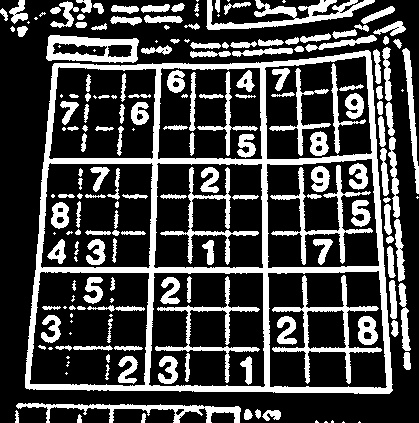
\includegraphics[width=\textwidth]{img/sht/input.jpeg}
      }
      \subcaptionbox{Wynik detekcji\label{fig:sht:output}}
      {
        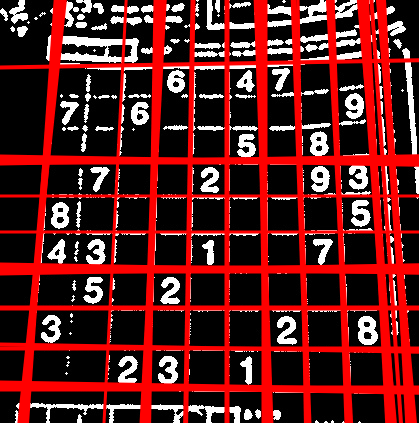
\includegraphics[width=\textwidth,trim=0 0 0 -1cm ]{img/sht/output.png}
      }%
      \end{minipage}%
  \hfill
  \begin{minipage}[c]{.475\linewidth}
    \subcaptionbox{Akumulator po głosowaniu\label{fig:sht:acc}}
      {
        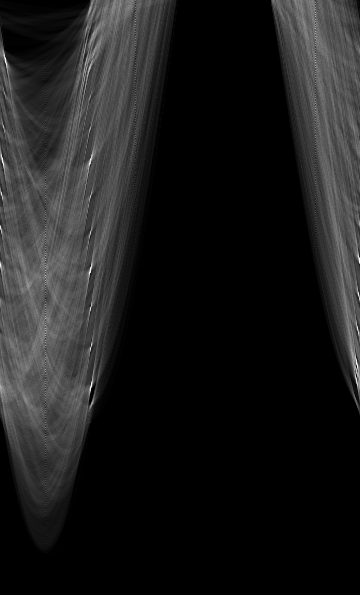
\includegraphics[width=\linewidth]{img/sht/equantial_acc.png}
      }%
  \end{minipage}%
  \caption{Wynik działania zaimplementowanego algorytmu SHT w~wariancie sekwencyjnym.}
  \label{fig:sht}
\end{figure}

\subsubsection{Circle Hough Transform}

Obraz testowy dla wariantu CHT przedstawiono na obrazie \ref{fig:cht:input}, a~wynik detekcji na \ref{fig:cht:output}. Poprzez rysowanie prostopadłych do kierunku krawędzi linii o~zakresie długości odpowiadającym długości wyszukiwanych promieni, w~procesie głosowania wygenerowany został akumulator przedstawiony na rysunku \ref{fig:cht:acc}. Jego rozmiar odpowiada rozmiarowi obrazu wejściowego, a~najjaśniejsze punkty są kandydatami na środki okręgów. Oprócz akumulatora dwuwymiarowego do detekcji promienia CHT wykorzystuje nieprzedstawiony tutaj akumulator jednowymiarowy, który bierze udział w~głosowaniu nad najlepszym promieniem. Dzieje się to osobno dla każdego kandydata na środek okręgu.

\begin{figure}
    \centering
    \begin{subfigure}{.475\linewidth}
          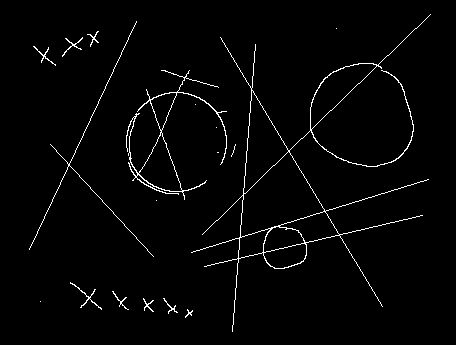
\includegraphics[width=\textwidth]{img/cht/input.png}
          \caption{Binarny obraz wejściowy}\label{fig:cht:input}
    \end{subfigure}%
    \hfill
    \begin{subfigure}{.475\linewidth}
      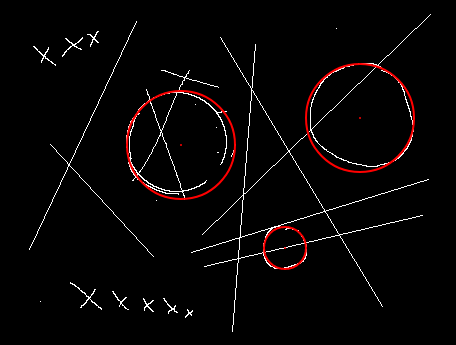
\includegraphics[width=\textwidth]{img/cht/output.png}
      \caption{Wynik detekcji}\label{fig:cht:output}
    \end{subfigure}% 
    \bigskip
    
    \begin{subfigure}{.475\linewidth}
      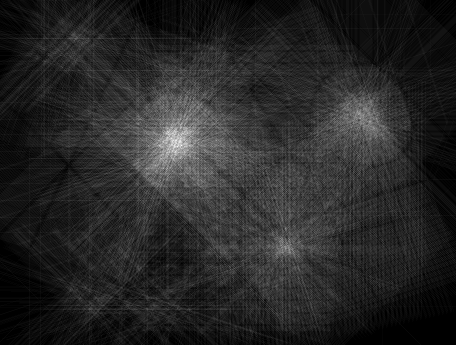
\includegraphics[width=\textwidth]{img/cht/sequential_acc.png}
      \caption{Akumulator po głosowaniu na środek okręgu}\label{fig:cht:acc}
    \end{subfigure}%
    \caption{Wynik działania zaimplementowanego algorytmu CHT w~wariancie sekwencyjnym.}
    \label{fig:cht}
  \end{figure}
  